\sectioncounter{46}

\section{统计初步}

\subsection{知识梳理}

在研究一些数据对象时, 把这些对象的全体称为总体, 每个对象称为个体. 研究的对象数量较多时, 只选取其中一部分来研究, 这一部分称为样本, 选取的过程称为抽样. 确定样本的特征后, 可以用这些特征来刻画总体.

从总体得到样本的抽样方法有: 简单随机抽样, 系统抽样, 分层抽样. 第一种方法适用于总体数量较少的时候. 第二种方法应用举例: 从编号为 $1\sim 100$ 的总体中抽取数量为 $5$ 的样本, 先把编号分为 $1\sim 20$, $21\sim 40$, $\cdots$, $81\sim 100$ 共 $5$ 组. 若从第 $1$ 组抽取 $2$ 号, 则后 $4$ 组依次抽取 $22$ 号, $42$ 号, $62$ 号和 $82$ 号. 第三种方法应用举例: 班里 $40$ 名同学, 男生 $16$ 人, 女生 $24$ 人. 现抽取 $10$ 人, 则应抽取男生 $4$ 人, 女生 $6$ 人, 即成比例抽取.

分析样本数据时, 有时可用频率分布直方图. 先将数据的取值范围分为若干个长度相等的区间, 再按区间将数据分组. 各组中数据的个数称为该组的频数, 频数与样本数量的比值称为该组的频率, 通常用小数表示. 确定频率后, 可以作出频率分布直方图. 注意直方图中用长方形的面积表示频率, 所以图中纵轴为 $\dfrac{\text{频率}}{\text{组距}}$.

常见的样本特征有平均数, 众数, 中位数和方差. 计算平均数时一般先找一个大致的基准点, 再计算各数与基准点差的平均值. 如 83, 87, 92, 95, 88 的平均值计算如下
\[\bar{x}= 90+\frac15(-7-3+2+5-2)= 89.\]
计算方差的公式为
\[s= \frac1n[(x_1-\bar{x})^2+(x_2-\bar{x})^2+\cdots
     + (x_n-\bar{x})^2],\]
由此可以看出方差表示的是数据的集中程度. 各数据同时增加 (或减少) 相同的数, 不会引起方差的改变. 如上面例子中 $5$ 个数的方差与 $-7$, $-3$, $2$, $5$, $-2$ 的方差相等. 此外可以证明, 若对数据 $x_1$, $x_2$, $\cdots$, $x_n$ 添加 $x_{n+1}$, 则 $x_{n+1}$ 离前 $n$ 个数的平均值越近, 新的 $n+1$ 个数的方差越小. 

有时样本的数据也会用茎叶图来表示, 即用茎和叶共同表示数据.

\lianxi
\begin{exercise}
    为了了解 $1000$ 名学生的学习情况, 采用系统抽样的方法从中抽取容量为 $40$ 的样本, 将学生编号为 $1$, $2$, $\cdots$, $1000$, 求抽样时分段的间隔.
\end{exercise}
\beginsolution
    $\dfrac{1000}{40}= 25$.
\endsolution

\begin{exercise}
    甲、乙两套设备生产的同类产品共 $4800$ 件, 采用分层抽样的方法从中抽取一个容量为 $80$ 的样本进行检测. 若样本中有 $50$ 件产品由甲设备生产, 求乙设备生产的产品总数.
\end{exercise}
\beginsolution
    设所求为 $x$, 由分层抽样的定义,
    \[\frac{50}{80}= \frac{4800-x}{4800},\quad x= 1800.\]
\endsolution

\begin{exercise}
    某班的全体学生参加英语测试, 成绩的频率分布直方图如图 \ref{fig-190629-1630} 所示, 数据的分组依次为: $[20, 40)$, $[40, 60)$, $[60, 80)$, $[80, 100]$. 若低于 $60$ 分的人数是 $15$, 求该班的学生人数.
    \begin{figure}[htb]
        \small
        \centering
        \begin{tikzpicture}[scale=0.7]
          \def\zftyb{0.007}%设定y轴比例,一定要先设
          \zftkz
          \zftzb{6}{成绩/分}{0.025}{20}{20}{5}
          %\zftzb{x长}{x标}{y长}{刻度始}{组距}{刻度数}
          \zft*{0}
          \zft{0.005}
          \zft{0.01}
          \zft{0.02}
          \zft{0.015}
        \end{tikzpicture}
       \caption{}\label{fig-190629-1630}
    \end{figure}
\end{exercise}
\beginsolution
    由图知, 低于 $60$ 分的频率为
    \[(0.005+ 0.01)\times 20= 0.3.\]
\endsolution
    
\begin{exercise}
    某中学有高中生 $1000$ 人, 初中生 $1500$ 人. 为了了解学生的学习情况, 用分层抽样的方法从该校学生中抽取一个容量为 $n$ 的样本. 若从高中生中抽取 $70$ 人, 求 $n$ 的值.
\end{exercise}
\beginsolution
    由分层抽样的定义,
    \[\frac{n}{40}= \frac{1000+1500}{1000},\quad n=100.\]
\endsolution

\subsection{要点导学\quad 各个击破}
\subsubsection{抽样方法}
\begin{example}
    某单位有职工 $52$ 人, 现将所有职工按 $1$, $2$, $\cdots$, $52$ 随机编号. 若采用系统抽样的方法抽取一个容量为 $4$ 的样本, 已知 $6$ 号职工在样本中, 求样本中另三位职工的编号.
\end{example}
\beginsolution
    编号分为 $4$ 组 (每组 $13$ 个数):
    \[1\sim 13,\quad 14\sim 26,\quad 
    27\sim 39,\quad 40\sim 52.\]
    因为 $6$ 号在第 $1$ 组, 所以第 $2$ 组取 $19$ 号, 第 $3$ 组取 $32$ 号, 第 $2$ 组取 $45$ 号.
\endsolution

\lianxi
\begin{exercise}
    某中学共有学生 $1000$ 人, 现从中随机抽取容量为 $200$ 的样本, 其中高中二年级被抽取的人数为 $64$, 求高中二年级的总人数.
\end{exercise}
\beginsolution
    设高中二年级的总人数为 $x$, 则
    \[\frac{x}{1000}= \frac{64}{200},\quad x=320.\]
\endsolution

\begin{exercise}
    某市有小型超市 $72$ 个, 中型超市 $24$ 个, 大型超市 $12$ 个. 现采用分层抽样的方法抽取 $9$ 个超市对其销售商品质量进行调查, 求应从小型、中型、大型超市分别抽取的个数. 
\end{exercise}
\beginsolution
    设应从小型、中型、大型超市分别抽取 $x$ 个、$y$ 个和 $z$ 个, 则
    \[x:y:z= 72:24:12,\quad x+y+z= 9,\]
    解得 $x=6$, $y=2$, $z=1$.
\endsolution

\subsubsection{总体分布的估计}
\begin{example}
    某校为了了解学生对食堂伙食的满意程度, 组织学生给食堂打分 (分数为整数, 满分为 $100$ 分), 从中随机抽取容量为 $120$ 的样本, 发现所有数据均在内. 现将这些分数的取值范围分成如下 $6$ 组:
    \[[40, 50),\ [50, 60),\ [60, 70),\ 
    [70, 80),\ [80, 90),\  [90, 100],\]
    并作出样本的频率分布直方图, 部分图形如图 \ref{fig-190629-1650} 所示.
    \begin{figure}[htb]
        \small
        \centering
        \begin{tikzpicture}[scale=0.7]
          \def\zftyb{0.007}%设定y轴比例,一定要先设
          %\zftkz
          \zftzb{8}{分数}{0.035}{40}{10}{7}
          %\zftzb{x长}{x标}{y长}{刻度始}{组距}{刻度数}
          %\zft*{0} % 无需标刻度
          \zft{0.005}
          \zft{0.015}
          \zft*{0}
          \zft{0.030}
          \zft{0.025}
          \zft{0.010}
        \end{tikzpicture}
       \caption{}\label{fig-190629-1650}
    \end{figure}
    
    (1) 写出第 $3$ 组 (对应 $[60, 70)$) 的频数, 并补全频率分布直方图;
    
    (2) 根据频率分布直方图估计样本的众数和平均数. 
\end{example}
\beginsolution
    (1) 第 $3$ 组的频数为
    \[1-(0.05+0.15+0.3+0.25+0.1)= 0.15,\]
    则频数为 $0.15\times 120= 18$, 对应图中矩形的高度为
    \[0.15\div 10= 0.015.\]

    (2) 众数在 $[70,80)$ 内, 可估计为 $75$. 取各组数据区间的中点, 并以 $75$ 为基准, 可算得平均数的估计值为 $73.5$.
\endsolution
    
\lianxi
\begin{exercise}
    从一批桔子中随机抽取 $50$ 个, 其质量的频数分布表如下:
    \[\begin{array}{c|cccc}
    \text{质量}/\text{g} & [80, 85) &[85, 90) 
        &[90, 95) &[95, 100) \\\hline
    \text{频数} &5 &10 &20 &15
    \end{array}\]
    
    (1) 根据频数分布表计算桔子的质量在 $[90, 95)$ 内的频率;
    
    (2) 用分层抽样的方法从质量在 $[80, 85)$ 和 $[95, 100)$ 内的桔子中共抽取 $4$ 个, 求其中质量在 $[80, 85)$ 内的桔子的个数.
\end{exercise}
\beginsolution
    (1) $\dfrac{20}{50}= 0.4$. (2) 设所求为 $x$, 则
    \[\frac{x}{5}= \frac{4}{5+15},\quad x=1.\]
\endsolution

\begin{exercise}
    为了研究某药物的疗效, 选取若干名志愿者进行临床试验, 所有志愿者的受药物影响的某种数据的分组区间为
    \[[12, 13),\ [13, 14),\ [14, 15),\ [15, 16),\ [16, 17],\] 
    并顺次编号为第一组, 第二组……第五组. 图 \ref{fig-190629-1700} 是根据试验数据制成的频率分布直方图.  已知第一组与第二组共有 $20$ 人, 第三组中没有疗效的有 $6$ 人, 求第三组中有疗效的人数. 
    \begin{figure}[htb]
        \small
        \centering
        \begin{tikzpicture}[scale=0.7]
          \def\zftyb{0.1}%设定y轴比例,一定要先设
          %\zftkz
          \zftzb{7.5}{数据}{0.43}{12}{1}{6}
          %\zftzb{x长}{x标}{y长}{刻度始}{组距}{刻度数}
          %\zft*{0} % 无需标刻度
          \zft{0.24}
          \zft{0.16}
          \zft{0.36}
          \zft{0.16}
          \zft{0.08}
        \end{tikzpicture}
       \caption{}\label{fig-190629-1700}
    \end{figure}
\end{exercise}
\beginsolution
    设所求为 $x$, 则
    \[\frac{6+x}{20}= \frac{0.36}{0.24+0.36},\quad x= 12.\]
\endsolution
    
\subsubsection{总体特征数的估计}
\begin{example}
    某车间共有 $30$ 名工人, 某日随机抽取 $6$ 名, 他们的日加工零件个数的茎叶图如下 (茎为十位数, 叶为个位数):
    \[\begin{array}{c|ccc}
      1& 7 & 9 & \\
      2 & 0 & 1 & 5 \\
      3 & 0 &  &
    \end{array}\]
    
    (1) 根据茎叶图计算样本均值;\qquad
    (2) 若规定日加工零件数大于样本均值的工人为优秀工人, 根据茎叶图推断该车间优秀工人的数量.
\end{example}
\beginsolution
    (1) 以 $20$ 为基准, 样本均值为
    \[20+ \frac16(-3-1+1+5+10)= 22.\]

    (2) $6$ 个样本中有 $2$ 名优秀工人, 占 $\dfrac13$, 故可估计 $30$ 名工人中有 $10$ 名优秀工人.
\endsolution

\lianxi
\begin{exercise}[s]
    在一次数学统考后, 某班随机抽取 $10$ 名同学的成绩进行样本分析, 获得成绩数据的茎叶图如下 (茎为十位数, 叶为个位数):
    \[\begin{array}{c|ccc}
      9 & 2 & 8 & 8\\
      8 & 5 & 5 &  \\
      7 & 4 & 4 & 4\\
      6 & 0 & 0 &
    \end{array}\]
    
    (1) 计算样本的平均成绩;\qquad
    (2) 现从样本里 $80$ 分以上的学生中随机抽出 $2$ 名, 求这 $2$ 名学生的成绩分别在 $[80, 90)$, $[90, 100]$ 内的概率.
\end{exercise}
\beginsolution
    (1) 平均成绩为
    \[80+ \frac{1}{10}(-20\times 2- 6\times 3
    + 5\times 2+ 12+ 18\times 2)= 80.\]

    (2) 样本里 $80$ 分以上的学生共 $5$ 人, 有 $2$ 人成绩在 $[80,90)$ 内, $3$ 人成绩在 $[90,100]$ 内, 故所求概率为
    \[2\times \frac25\times \frac35= \frac{12}{25}.\]
\endsolution

\subsubsection{课堂评价}
\begin{exercise}
    某学校高一年级男生人数占该年级学生人数的 $40\%$, 在一次考试中, 男生、女生的平均分分别是 $75$ 和 $80$, 求这次考试该年级学生的平均分.
\end{exercise}
\beginsolution
    女生人数占该年级学生人数的 $60\%$, 则所求为
    \[75\times 40\%+ 80\times 60\%= 78.\]
\endsolution

\begin{exercise}
    某工厂甲、乙、丙三个车间生产了同一种产品, 数量分别为 $120$ 件、$80$ 件、$60$ 件. 为了解它们的产品质量, 用分层抽样的方法抽取了一个容量为 $n$ 的样本, 其中从丙车间的产品中抽取了 $3$ 件, 求 $n$ 的值.
\end{exercise}
\beginsolution
    $\dfrac{3}{60}= \frac{n}{120+80+60}$, $n=13$.
\endsolution

\begin{exercise}
    某种树木底部周长 (单位: $\text{cm}$) 的取值范围是 $[80, 130]$, 抽测 $60$ 株树木, 它们的底部周长的频率分布直方图如图 \ref{fig-190629-1710} 所示, 求其中底部周长小于 $100\,\text{cm}$ 的树木数量.
    \begin{figure}[htb]
        \small\centering
        \begin{tikzpicture}[scale=0.7]
          \def\zftyb{0.008}%设定y轴比例,一定要先设
          %\zftkz
          \zftzb{7.5}{底部周长/cm}{0.036}{80}{10}{6}
          %\zftzb{x长}{x标}{y长}{刻度始}{组距}{刻度数}
          %\zft*{0} % 无需标刻度
          \zft{0.015}
          \zft{0.025}
          \zft{0.030}
          \zft{0.020}
          \zft{0.010}
        \end{tikzpicture}
       \caption{}\label{fig-190629-1710}
    \end{figure}
\end{exercise}
\beginsolution
    $60\times 10\times (0.015+0.025)= 24$.
\endsolution
    
\subsection{课后练习}
\begin{exercise}
    某工厂生产 $A,B,C$ 三种不同型号的产品, 三种产品数量之比为 $2:3:4$. 现采用分层抽样的方法从中抽出一个容量为 $n$ 的样本, 样本中 $A$ 型号的产品有 $16$ 件, 求 $n$ 的值.
\end{exercise}
\beginsolution
    $\dfrac{16}{2}= \dfrac{n}{2+3+4}$, $n=72$.
\endsolution

\begin{exercise}
    设数据 $x_1$, $x_2$, $x_3$, $x_4$, $x_5$, $3$ 平均数是 $3$, 求 $x_1$, $x_2$, $x_3$, $x_4$, $x_5$ 的平均数.
\end{exercise}
\beginsolution
    设所求为 $x$, 则
    \[\frac{5x+3}{6}= 3,\quad x=3.\]
\endsolution

\begin{exercise}
    某学员在一次射击测试中射靶 $10$ 次, 命中环数分别为 
    \[7,\ 8,\ 7,\ 9,\ 5,\ 4,\ 9,\ 10,\ 7,\ 4,\]
    求命中环数的平均数和方差.
\end{exercise}
\beginsolution
    以 $7$ 为基准, 平均值为
    \[7+ \frac{1}{10}(1+2-2-3+2+3-3)= 7,\]
    方差为
    \[\frac{1}{10}[1^2+2^2+(-2)^2+(-3)^2+
    2^2+3^2+(-3)^2]= 4.\]
\endsolution

\begin{exercise}
    为了了解某地区高三学生的体重, 抽查了该地区 $100$ 名高三男生的体重 (单位: $\text{kg}$), 得到频率分布直方图如图 \ref{fig-190629-1720} 所示. 求这 $100$ 名学生中体重在 $[56, 64)$ 内取值的人数.
    \begin{figure}[htb]
        \small\centering
        \begin{tikzpicture}[scale=0.7]
          \def\zftyb{0.02}%设定y轴比例,一定要先设
          %\zftkz
          \zftzb{13}{体重/kg}{0.09}{54}{2}{12}
          %\zftzb{x长}{x标}{y长}{刻度始}{组距}{刻度数}
          \zft*{0.01}
          \zft{0.03}
          \zft{0.05}
          \zft*{0.05}
          \zft{0.07}
          \zft*{0.09}
          \zft*{0.062}
          \zft*{0.048}
          \zft*{0.042}
          \zft*{0.028}
          \zft*{0.02}
        \end{tikzpicture}
       \caption{}\label{fig-190629-1720}
    \end{figure}   
\end{exercise}
\beginsolution
    $100\times 2\times (0.03+0.05\times 2+ 0.07)= 40$.
\endsolution

\begin{exercise}
    在一次比赛中, 将某选手的 $9$ 个得分 (均为整数) 去掉 $1$ 个最高分, 去掉 $1$ 个最低分, 则 $7$ 个剩余分数的平均分为 $91$. 现场做的 $9$ 个分数的茎叶图后来有一个数据模糊, 无法辨认, 在图中以 $x$ 表示, 求前述 7 个剩余分数的方差.
    \[\begin{array}{c|ccccccc}
      8 & 7 & 7 & &&&&\\
      9 & 4 & 0 & 1 & 0 & x & 9 & 1
    \end{array}\]
\end{exercise}
\beginsolution
    显然最低分为 $87$, 最高分为 $99$. 考虑 $7$ 个剩余分数的平均分, 以 $91$ 为基准, 则
    \[\frac17[-4+3-1-1+(x-1)]= 0,\quad x= 4,\]
    所以方差为
    \[\frac17[(-4)^2+3^2+(-1)^2+(-1)^2+3^2]= \frac{36}{7}.\]
\endsolution

\begin{exercise}
    为了考察某校各班参加课外书法小组的人数, 从全校随机抽取 5 个班级, 将每个班级参加该小组的人数作为样本数据. 已知样本平均数为 $7$, 样本方差为 $4$, 且样本数据互不相同, 求样本数据中的最大值.
\end{exercise}
\beginsolution
    设 $5$ 个数据为 $7+x_1$, $7+x_2$, $7+x_3$, $7+x_4$, $7+x_5$, 其中 $x_i$, $i=1,2,\cdots,5$ 均为整数且互不相同, 则
    \[\begin{gathered}
        x_1+x_2+x_3+x_4+x_5= 0,\\
        \frac{1}{5}(x_1^2+x_2^2+x_3^2+x_4^2+x_5^2)= 4.
    \end{gathered}\]
    考虑 $|x_i|$, $i=1,2,\cdots,5$, 容易知道, 最小的情形是 $0$, $1$, $1$, $2$, $2$, 此时上述第 $2$ 式已成立. 不妨设 $x_1<x_2<x_3<x_4<x_5$, 则
    \[x_1= -2,\ x_2= -1,\ x_3= 0,\ x_4=1,\ x_5=2,\]
    所以样本数据中的最大值为 $9$.
\endsolution


\begin{exercise}
    某人在如图 \ref{fig-190629-1600} 所示的直角边长为 $4\,\text{m}$ 的三角形地块的每个格点 (指横、纵直线的交叉点及三角形的顶点) 处都种了一株相同品种的作物. 根据历年的种植经验, 一株该种作物的年收获量 $Y$ (单位: kg) 和与它的“相近”作物株数 $X$ 之间的关系如下表所示:
    \[\begin{array}{c|cccc}
      X &1 &2 &3 &4 \\\hline
      Y &51 &48 &45 &42
    \end{array}\]
    这里, 两株作物“相近”是指它们之间的距离不超过 $1\,\text{m}$. 补全 $Y$ 的频数分布表, 并求所种作物的平均年收获量. 
    \[\begin{array}{c|cccc}
      Y & 51 & 48 & 45 & 42 \\
      \hline
      \text{频数} & &4 & &
    \end{array}\]
    \begin{figure}[htb]
        \small
        \centering
        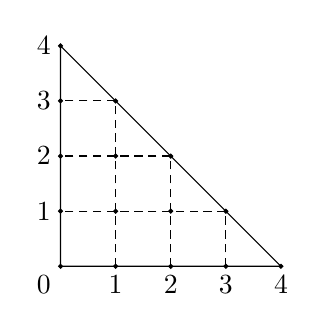
\begin{tikzpicture}[scale=0.7]
          \def\layer{4}
          \foreach \y in {0,...,\layer}
            \foreach \x in {\y,...,\layer}
            {\draw[fill=black] (\layer-\x,\y) circle (1pt);}
          
          \draw (0,0) node[anchor=north east] {$0$};
          \foreach \x in {1,...,4}
            {\draw (\x,0) node[below] {$\x$} (0,\x) node[left] {$\x$};}
          
          \foreach \x in {1,2,3}
            {\draw[densely dashed] (\x,0)--(\x,4-\x)--(0,4-\x);}
          
          \draw (0,0)--(\layer,0)--(0,\layer)--(0,0);
        \end{tikzpicture}
        \caption{}\label{fig-190629-1600}
    \end{figure}
\end{exercise}
\beginsolution
    $Y$ 的频数分布表为 
    \[\begin{array}{c|cccc}
      Y & 51 & 48 & 45 & 42 \\
      \hline
      \text{频数}  & 2 & 4 & 6 & 3
    \end{array}\]
    以 $48$ 为基准计算平均收获量,
    \[48+ \frac{1}{15}(2\times3- 6\times3- 3\times6)
    = 46\,\text{kg}.\]
\endsolution
